\section{Tree time!}
\label{sec:tree_time_}

\begin{frame}
	\frametitle{Tree time}
	\begin{center}
		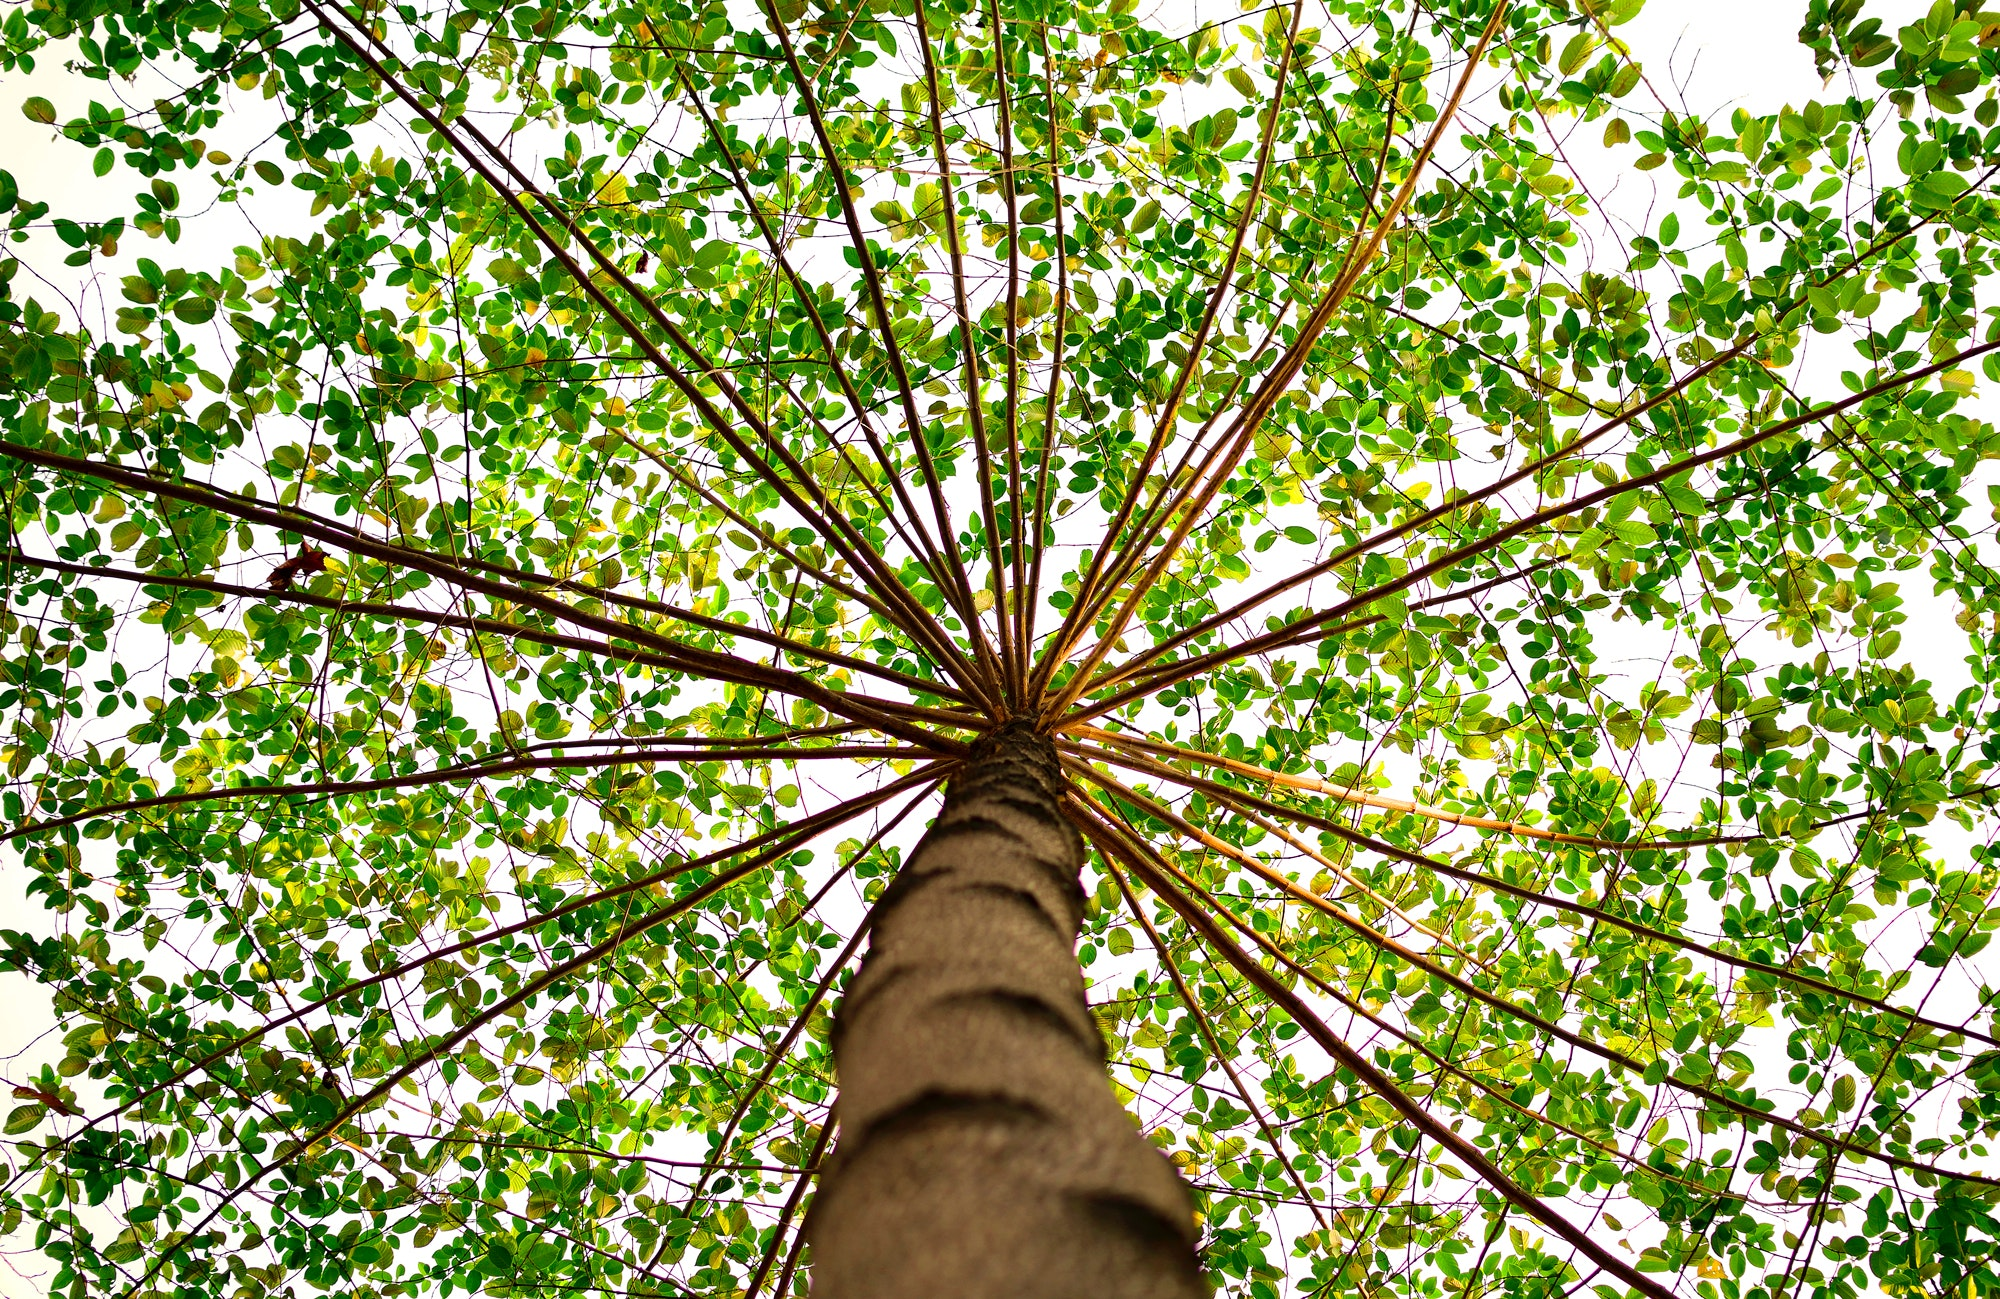
\includegraphics[width=0.6\textwidth]{figures/tree.jpg}\\
		\hspace*{15pt}\hbox{\scriptsize Image By:\thinspace{\itshape George achik}}
		% https://commons.wikimedia.org/wiki/File:Last_summer_time_tree_and_evening_time,_In_Srimongol,_Bangladesh.jpg
	\end{center}
\end{frame}

\begin{frame}
	\frametitle{Properties}
	\begin{columns}
		\column{0.405\textwidth}
			\begin{tikzpicture}[
				level distance = 2.5em,
				level 1/.style={sibling distance=9em},
				level 2/.style={sibling distance=4.5em},
				level 3/.style={sibling distance=2.25em},
			]
			\node[ellipse,onslide=<5>{draw=red}] (t1) {\alert<1,6>{root}}
				child { node[ellipse] {\alert<2,4,5>{child 1}}
					child { node[ellipse] {\alert<3,5>{leaf 1}}}
				}
				child { node[ellipse] {\alert<2,4,5,6>{child 2}}
					child { node[ellipse] {\alert<3,5>{leaf 2}}}
					child { node[ellipse,onslide=<6>{draw=red}] {\alert<3,5>{leaf 3}}}
					child { node[ellipse] {\alert<3,5>{leaf 4}}}
				};
			\end{tikzpicture}
		\column{0.555\textwidth}
		\begin{itemize}
			\item The \textit{root node} is the node that has no \textit{parent}.
				\pause
			\item A node can have \textit{children}.
				\pause
			\item A node without children is called a \textit{leaf}.
				\pause
			\item Two nodes with the same \textit{parent} are \textit{siblings}.
				\pause
			\item \textit{Descendants} are found by repeatedly following child-relations.
				\pause
			\item \textit{Ancestors} are found by repeatedly following parent-relations.
		\end{itemize}
	\end{columns}
\end{frame}

\begin{frame}
	\frametitle{Quick check}
	
	\begin{columns}
		\column{0.405\textwidth}
			\begin{tikzpicture}[
				level distance = 2.5em,
				level 1/.style={sibling distance=2em},
				level 2/.style={sibling distance=4.5em},
				level 3/.style={sibling distance=2.25em},
			]
			\node[ellipse] (t1) {r}
				child { node[ellipse] {k}
					child { node[ellipse] {d}}
				}
				child { node[ellipse] {a} }
				child { node[ellipse] {b} }
				child { node[ellipse] {e} 
					child { node[ellipse] {g} }
					child { node[ellipse] {h}
						child { node[ellipse] {i}}
					}
				}
				child { node[ellipse] {f} };
			\end{tikzpicture}
		\column{0.555\textwidth}
		\pause
			\begin{questionblock}{Let's see if that was a clear}
				Let $c(v)$ be the set of children of $v$.\\
				Let $d(v)$ be the set of descendants of $v$.\\
				Let $s(v)$ be the set of siblings of $v$.\\
				Let $a(v)$ be the set of ancestors of $v$.\\
				Let $p(v)$ be the parent of $v$.\\
				What is: $|c(k)| + |d(p(g))| + \sum\limits_{v \in a(h)} |s(v)|$?
				\begin{multicols}{2}
				\begin{enumerate}[A.]
					\item 4
					\item 8
					\item 12
					\item I don't know
				\end{enumerate}
			\end{multicols}
			\end{questionblock}
	\end{columns}
	\pause
	\vspace{-5pt}
	\begin{answerblock}{Arithmetic time}
		$c(k) = \{d\}$, $p(g) = e$, $d(e) = \{g,h,i\}$, $a(h) = \{r,e\}$, $s(r) = \emptyset$, $s(e) = \{k,a,b,f\}$. So the
		final answer is: $1+3+4=8$.
	\end{answerblock}
\end{frame}
